\documentclass[authordate, empirical]{jote-new-article}

\usepackage{caption}

\usepackage{tabularx}

\usepackage{graphicx}

\usepackage{hyperref}

\usepackage[backend=biber,style=apa]{biblatex}

\addbibresource{bibliography.bib}

\jotetitle{Attentional bias and tobacco smoking frequency: A reflection on Bartlett et al. (2022)}
\keywordsabstract{attentional bias, tobacco, visual probe task, reliability}
\abstracttext{In this manuscript, I provide a reflection on Bartlett et al.'s (2022) study, \emph{No Meaningful Difference in Attentional Bias Between Daily and Non-Daily Smokers}. I begin with an overview of attentional bias and its measurement in addiction research, followed by a summary of the study by Bartlett et al. (2022). I then discuss the broader implications of this research, with particular emphasis on methodological implications for the field. Finally, I outline directions for future research that address limitations of previous studies and seek to integrate attentional bias mechanisms into contemporary value-based decision-making frameworks.}
\runningauthor{Copeland}
\jname{Journal of Trial \& Error}
\jyear{2025}
\paperdoi{10.36850/f7a7-4c8d}
\paperreceived{June 9, 2025}
\author[1]{\mbox{Amber Copeland\orcid{0000-0003-4634-3343}}}
\affil[1]{University of Sheffield, Sheffield, England}
\corremail{\href{mailto:a.copeland@sheffield.ac.uk}{a.copeland@sheffield.ac.uk}}
\corraddress{University of Sheffield}
\runningauthor{Copeland}
\paperaccepted{August 21, 2025}
\paperpublished{October 28, 2025}
\paperpublisheddate{2025-10-27}
\jwebsite{https://journal.trialanderror.org}

\begin{document}
\begin{frontmatter}
  \maketitle
  \begin{abstract}
    \printabstracttext
  \end{abstract}
\end{frontmatter}



	\section{Attentional bias in addiction research: A brief overview}



	Attentional bias refers to the tendency for motivationally salient cues to “capture” and “hold”\emph{ }selective attention. Theoretical models of addiction predict that attentional bias toward substance-related cues (e.g., a lit cigarette or a bottle of alcohol) plays a key role in the development and maintenance of addictive behavior (for a review, see Field \& Cox, 2008). Over time, however, the field has become increasingly characterized by mixed findings, with updated accounts suggesting that attentional bias is neither consistently linked to individual differences in substance use nor as causally influential as previously assumed (Creswell \& Skrzynski, 2021; Field et al., 2016).



	Addiction researchers have typically relied on reaction time outcomes from computerized laboratory tasks to make \emph{indirect} inferences about underlying cognitive processes (Field \& Cox, 2008). Among these methods, the addiction Stroop (Cox et al., 2006) and visual probe task (also termed the dot-probe task\footnote{ From this point onwards only the term “visual probe task” will be used.}; MacLeod et al., 1986) are commonly used to quantify attentional bias by calculating differences in reaction times to substance-related versus neutral cues. One acknowledged limitation is the noisiness of reaction time measures, which may reflect multiple processes and confound assessments of attentional bias (Field \& Cox, 2008; Pennington et al., 2021). As a result, eye-tracking technology which captures eye movements and fixations at the millisecond level has been used to provide more \emph{direct }measurements of attentional bias (Bollen et al., 2024; Rahmani et al., 2024; Schröder \& Mühlberger, 2023; Soleymani et al., 2020).



	\section{Summary of Bartlett et al. (2022)}



	Bartlett et al. (2022) conducted a pre-registered (\url{https://osf.io/t3xw8/}) online study examining attentional bias differences between daily (\emph{n} = 106) and non-daily (\emph{n} = 60) smokers who were recruited via Prolific—an online recruitment platform. It was hypothesized that non-daily smokers would demonstrate greater attentional bias toward smoking-related images compared to daily smokers. Participants self-reported their tobacco use patterns before completing a visual probe task, in which they were simultaneously presented with paired images on a computer screen (one smoking-related, e.g., a person holding a cigarette, and one matched control image, e.g., a person holding a fork). After a brief interval (either 200ms or 500ms), both images disappeared and were replaced by a visual probe appearing in the location of one of the pictures. Reaction time to this probe served as an index of attentional bias, with faster responses to probes replacing smoking-related images indicating greater attentional bias to those stimuli.



	Contrary to predictions, a 2 x 2 mixed ANOVA revealed no support for the core hypothesis, as non-daily smokers did not demonstrate greater attentional bias toward smoking images compared to daily smokers. Exploratory equivalence testing further indicated that the observed effects were statistically equivalent to zero. Importantly, the study found poor psychometric properties for the visual probe task, with both Cronbach's alpha and split-half reliability estimates indicating inadequate internal consistency for the attentional bias measure across both stimulus onset asynchrony (SOA) conditions (200ms and 500ms). Based on these findings, Bartlett et al. (2022) concluded that stable trait-like differences in attentional bias between smoking groups are unlikely to exist, and that the visual probe task demonstrates insufficient reliability for repeated testing or investigating individual differences.



	\section{Contributions to research on attentional biases in addiction}



	\subsection{Methodological implications}



	The study by Bartlett et al. (2022) contributes to a large body of evidence (Ataya et al., 2012; Field \& Christiansen, 2012; Field et al., 2016; Jones et al., 2018) emphasizing inadequate reliability of the visual probe task. To elaborate, both Cronbach's alpha and split-half reliability estimates indicated poor internal consistency for both 200ms (α = .29; \emph{r} = .56) and 500ms (α = .19; \emph{r} = .47) SOA conditions. Bartlett et al. (2022) therefore contribute to growing evidence questioning the continued use of attentional bias measures with suboptimal psychometric properties, particularly the visual probe task.



	In addition, I believe that Bartlett et al. (2022) exemplify open, robust, and transparent scientific practices that warrant recognition and carry important methodological implications for the field, as discussed below.



	First, Bartlett et al. (2022) pre-registered their study design, hypotheses, and analysis strategy on the Open Science Framework (\href{https://osf.io/}{https://osf.io/}) prior to data collection, and in doing so clearly distinguished between confirmatory and exploratory analyses. Their transparency represents a considerable methodological strength. This helps mitigate researcher degrees of freedom (Wicherts et al., 2016) because specific analytic decisions are disclosed in advance. Moreover, it is particularly important given the substantial variability and wide range of analytic decisions involved in processing reaction time outcomes in attentional bias research. For example, Jones et al. (2021) estimated that there are \textasciitilde{}768 possible analysis pipelines for the alcohol Stroop task alone. Although Bartlett et al. (2022) focuses on tobacco-related attentional bias, evidence from the alcohol literature suggests that pre-registration is exceedingly rare; in a recent review, fewer than 2\% of studies on attentional bias adhered to pre-registration protocols (Pennington et al., 2021).



	Second, an \emph{a priori} power analysis was conducted to determine the appropriate sample size required to detect the anticipated effect. Statistical power (the ability to detect true experimental effects) is a known contributor to the ongoing reproducibility crisis in science, particularly in psychology (Munafò et al., 2017; Nosek et al., 2022). Systematic reviews on the topic of attentional bias have identified the absence of \emph{a priori} power analyses as a key methodological limitation affecting research quality (Bollen et al., 2022; Farr et al., 2024), thereby complicating the interpretation of inconclusive findings that may be attributable to low statistical power. Consistent with the approach taken by Bartlett et al. (2022), future attentional bias research would benefit from routinely conducting \emph{a priori} power analyses or, at a minimum, providing a clear justification for the selected sample size (Lakens, 2022).



	Third, by using equivalence testing (Lakens et al., 2018), Bartlett et al. (2022) propose to overcome a common issue in psychological research where non-significant results are conclusively interpreted as evidence of “no effect” (Altman \& Bland 1995; Lakens, 2017). Equivalence testing enables researchers to statistically reject the presence of effects smaller than a predefined smallest effect size of interest, allowing them to demonstrate that the difference between two groups is not practically meaningful, rather than merely showing that one group is not significantly different from the other. However, while equivalence testing provides a stronger inference than simply failing to reject the null hypothesis, its effectiveness depends critically on establishing a well-justified smallest effect size of interest (SESOI), which is often subjective (Riesthuis \& Cribbie, 2025). Although not employed by Bartlett et al. (2022), I note that alternative methods, such as Bayesian approaches (Wagenmakers et al., 2018), can aid in statistical interpretation by quantifying the strength of evidence for both null and alternative hypotheses.



	Finally, Bartlett et al. (2022) made their adaptation of the visual probe task publicly available (\href{https://gorilla.sc/openmaterials/85021}{https://gorilla.sc/openmaterials/85021}). This promotes reproducibility, removes the need for researchers to contact the authors for access, and enhances transparency around key methodological decisions, such as stimuli used (Pennington et al., 2021). A minor caveat is that the smoking and non-smoking images used by Bartlett et al. (2022) were developed internally. While they provide a Gorilla link, it redirects to a task preview which suggests that researchers wanting to examine the actual stimuli may need to clone the task and create an account. This could present a barrier to reproducibility. Furthermore, reviews have highlighted substantial methodological variability in how the visual probe task is administered, along with inconsistent reporting on methodological specifics (Zhang et al., 2019). A key consequence of this heterogeneity is that it often prevents meta-analyses, thereby creating a barrier to effective evidence synthesis (Farr et al., 2024). I commend Bartlett et al. (2022) for openly disclosing a coding error within their adaptation of the visual probe task; this not only shows scientific integrity, but also helps normalize the acknowledgment of errors in the field.



	Overall, Bartlett et al. (2022) make a valuable contribution to attentional bias research by demonstrating methodological rigor and the use of robust statistical techniques. Their commitment to transparency, including the provision of open materials, strengthens the reproducibility of their approach and offers a strong foundation for future attentional bias research on to build upon.



	\subsection{Theoretical implications}



	A critical consideration in empirical research is that data derived from tasks lacking reliability cannot (or should not) be used as strong evidence for or against theoretical frameworks. To elaborate, when the task exhibits poor reliability, any observed effects may reflect measurement error or noise rather than compelling support or contradiction of theoretical claims. I therefore approach the extension of findings from Bartlett et al. (2022) to theoretical implications with caution and encourage readers to do the same.



	Bartlett et al. (2022) interpret the absence of group differences in attentional bias toward tobacco cues between daily and non-daily smokers as consistent with contemporary accounts of attentional bias (Field et al., 2016). These accounts emphasize that attentional bias is not a stable, trait-like phenomenon but rather a dynamic process that fluctuates in response to current motivational states shaped by environmental and internal factors. Indeed, empirical studies have demonstrated fluctuations in substance-related attentional biases in relation to broader contextual factors, such as subjective craving and stress (Begh et al., 2016; Bollen et al., 2022; Bollen et al., 2024; Schröder \& Mühlberger, 2023). As Bartlett et al. (2022) compared two groups that differ in the severity of tobacco use at a single point in time, and because attentional bias is not stable, this may explain why no significant difference was observed. However, there has long been recognition that in smokers, evidence is mixed as to whether attentional bias can distinguish between quantity and frequency of substance use (Field \& Cox, 2008), and indeed this is supported by prior empirical studies (Wilcockson et al., 2021). To more convincingly provide evidence in support of contemporary theory, several methodological improvements can be made, which I outline in the next section.



	\section{Avenues for future research on attentional biases in addiction}



	Addressing the methodological limitations of previous studies (including Bartlett et al., 2022) presents an opportunity for advancing our understanding of attentional biases in addiction. Firstly, measuring attentional bias at a single timepoint may have limited sensitivity to within-subject fluctuations according to craving level and perceived value of tobacco at testing time (Field et al., 2016), which might have masked between-groups differences. Future research could make use of repeated testing over time and in ecologically valid settings. Indeed, technological advances increasingly enable real-time data collection, with methods such as ecological momentary assessment (EMA) becoming more accessible through user-friendly tools and tutorials (Dora et al., 2024).



	Secondly, categorizing participants solely by daily smoking status may have overlooked important variation in levels of tobacco use.\footnote{ In Bartlett et al. (2022), participants answered the question “Do you usually smoke cigarettes every day?” Daily smokers were those who responded yes, and non-daily smokers were those who responded no.} Differences in how studies define groups based on frequency of use represent a key consideration when attempting to reconcile inconsistent findings in the broader literature (Field \& Cox, 2008). Future research could make use of more granular screening methods, could provide a more sensitive measure of use severity, as well as enhance group differentiation. For example, Prolific offers an embedded pre-screen tool with specific questions about frequency of tobacco use (Figure 1), as used in prior research (e.g., Copeland et al., 2025).



	\begin{figure}
		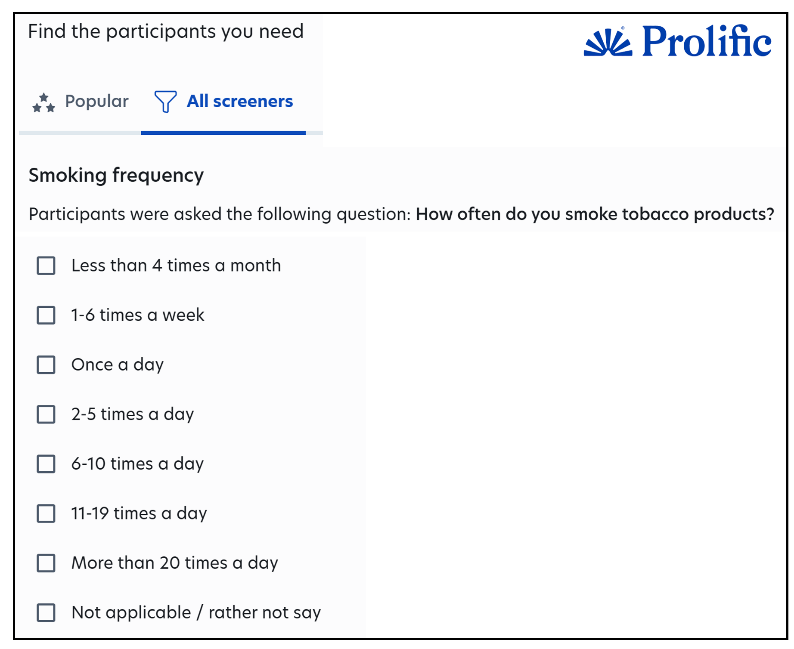
\includegraphics[width=\linewidth]{media/image1.png}

		\caption{An example of an embedded pre-screen tool offered by Prolific (\url{https://www.prolific.com/}) to filter participants according to varying levels of tobacco use.}

		\label{fig:rId11}


	\end{figure}





	\subsection{Toward more reliable attentional bias tasks}



	As I described earlier, findings from Bartlett et al. (2022) add to an existing body of evidence (Ataya et al., 2012; Field \& Christiansen, 2012; Field et al., 2016; Jones et al., 2018) demonstrating poor reliability of the visual probe task.



	To address this issue, one potential approach is to employ \emph{MouseView}, an open-source software designed to measure attentional bias. This tool is marketed as providing "eye tracking without the eyes" (Anwyl-Irvine et al., 2022). Using this software, researchers can develop decision-making tasks which feature initially blurred (to mimic peripheral vision) side-by-side images. Participants reveal portions of images by moving a small, mouse-controlled circular aperture that unblurs the viewed area. MouseView tracks the coordinates of the aperture viewing window to identify where and how long participants viewed images for, which provides a measure analogous to fixation duration or dwell time in eye tracking research (Woronko et al., 2023). Crucially, dwell time differences recorded with MouseView have been found to correlate highly, and to be equally as reliable, as those obtained through eye tracking (Anwyl-Irvine et al., 2022). This approach can offer eye-tracking-like precision with the practicality of remote testing, and can be implemented on user-friendly task platforms such as Gorilla (Anwyl-Irvine et al., 2020) which was used to build the task used in Bartlett et al. (2022). Combined with recruitment platforms like Prolific, this enables scalable, high-quality (Peer et al., 2022) data collection without the challenges of home-based eye-tracking. While this software has been used to study attentional biases across various psychological domains (Anwyl-Irvine et al., 2022; McNamara et al., 2025; Milani et al., 2025; Woronko et al., 2023), to the best of my knowledge, this has yet to be extended to research on attentional bias in the context of addiction.



	\subsection{Alternative approaches to quantifying attentional bias using behavioral data}



	A core take-home message from Bartlett et al. (2022, p. 2) is that “response time outcomes from the [visual probe] task should not be used when studying individual differences or measuring changes in attentional bias…” In the current section, I explain how the drift-diffusion model (Ratcliff \& McKoon, 2008) can be fitted to routinely collected behavioral data from the visual probe task to estimate underlying cognitive processes.



	Commonly used approaches quantify attentional bias using average differences in reaction time. For example, in alcohol research alone, this method accounted for 72.06\% of attentional bias measures reported (Pennington et al., 2021). However, when used as the outcome measure of interest, this assumes that systematic differences in reaction time are driven only by the construct under investigation, whereas it is known that various cognitive (e.g., response caution) and motor processes (e.g., executing a response, such as a key press) influence reaction time simultaneously (Hedge et al., 2018).



	When fitted to behavioral data, the drift-diffusion model provides principled reconciliation of reaction time and accuracy (both of which are collected in the visual probe task) to estimate different cognitive processes that determine overt behavior (White et al., 2016). These processes are captured by parameters recovered from the model, each with well-established psychological interpretations (Stafford et al., 2020): \emph{evidence accumulation rate} (also known as drift rate), reflecting the rate at which momentary evidence is accumulated; \emph{response threshold}, indexing participant caution via their speed--accuracy trade-off (SATO); and \emph{non-decision time}, representing perceptual encoding and motor execution processes. Crucially, the drift-diffusion model disentangles the different processes that determine decision-making. Indeed, research on the topic of anxiety has found that fitting this model to data from the visual probe task yields more reliable, precise, and sensitive attentional bias metrics (Price et al., 2019).



	Another methodological benefit is that fitting the drift-diffusion model, compared to relying on observed behavioral data (e.g., reaction time), has been shown to enhance statistical power when comparing two groups—without the need for additional participants or task trials (Stafford et al., 2020). The combination of more precise and sensitive measures, alongside enhanced power, may correspond to ability to uncover robust between-subject (or individual difference) effects (van Ravenzwaaij \& Oberauer, 2009).



	\subsection{Interpreting attentional bias through the lens of value-based decision making}



	In this next section, inspired by my own research interests and expertise, I speculate on the role of attentional bias through the lens of contemporary value-based decision-making (VBDM) accounts (Berkman et al., 2017; Berkman, 2018), particularly those applied to the study of addiction (Copeland et al., 2021; Field et al., 2020). This has been alluded to in previous accounts: Field et al. (2016) propose, for example, that both attentional bias and behavior are influenced by the incentive value of the substance at a given moment. Nevertheless, previous work has not fully integrated these concepts within a computational framework.



	Relative substance value is a key underlying mechanism of addiction vulnerability (Copeland et al., 2021; Field et al., 2020; Hogarth \& Field, 2020), and it can be influenced by various factors, including attentional bias (Field et al., 2016). Previous studies (Rose et al., 2013; Rose et al., 2018) demonstrated that experimental devaluation of alcohol (via taste manipulation) reduced the proportion of initial fixations and percent dwell time on alcohol cues, and that this reduction in attentional bias mediated the effect of the manipulation on actual alcohol consumption. However, these findings offer little insight into the internal cognitive mechanisms that precede decisions made, or the role of attention in these moment-to-moment, dynamic processes.



	VBDM offers a framework for modelling the internal cognitive processes involved in momentary decision-making. According to VBDM, when a person is making a decision, the value of each response option is determined as the weighted sum of choice-relevant attributes which can vary across individuals, context, and time (Berkman, 2018). The response option higher in value is subsequently acted upon—a process which can be estimated by fitting the drift-diffusion model (previously described) to data from behavioral tasks that involve value judgements. Extensions of the drift-diffusion model have enabled researchers studying value-based choice to incorporate eye-tracking data into the modelling of decision-making processes (March \& Gluth, 2025; Yang \& Krajbich, 2023). The attentional drift-diffusion model (aDDM) posits that gaze modulates evidence accumulation during decision-making, such that more evidence is accumulated for items being fixated than for those not being looked at (Krajbich et al., 2010).



	I propose that this offers a unique opportunity to integrate existing research on attentional bias within VBDM accounts of addiction, which emphasize the role of moment-to-moment evaluations in determining substance use. It may be that attentional bias towards substance-related stimuli inflates perceived value via an increase in the evidence accumulation process (see Figure 2), which in turn increases the likelihood of a substance-related decision being made. However, as with other contemporary models of attentional bias (Field et al., 2016), this process is dynamic and context-dependent, which may obscure between-subject differences depending on the timing of assessment. Overall, combining robust experimental techniques, such as those employed by Bartlett et al. (2022), eye-tracking, and computational modelling, is likely to provide new insights into the dynamic role of attentional bias in addiction.



	\begin{figure}
		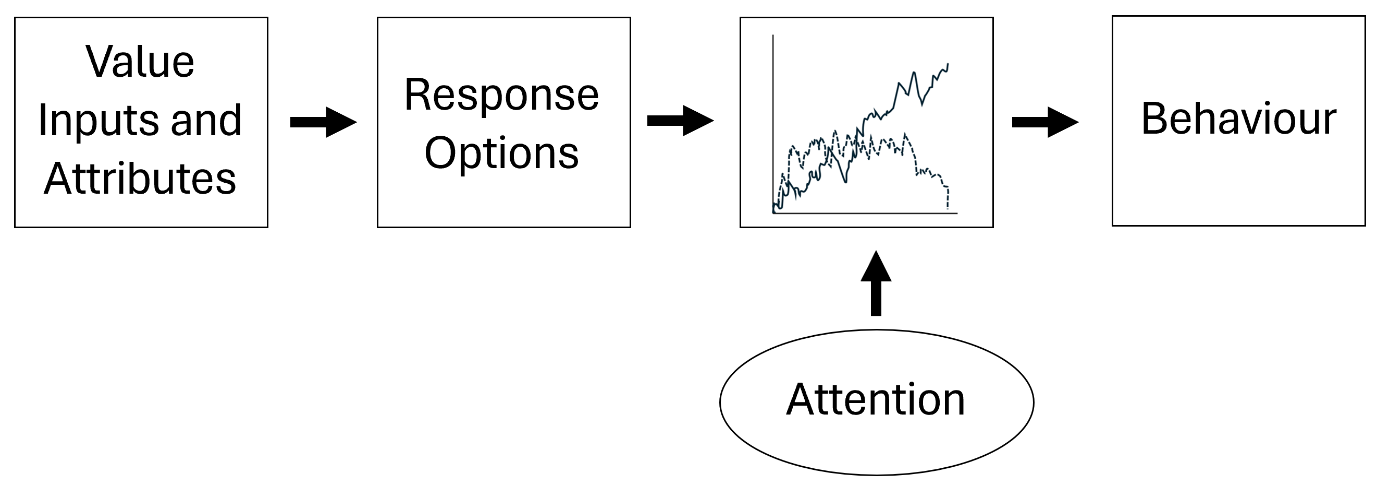
\includegraphics[width=\linewidth]{media/image2.png}

		\caption{A depiction of value-based decision-making. The value of each response option is computed as a weighted sum of its choice-relevant attributes. Response options are assigned an overall value, and then through a value-to-evidence accumulation process a decision is made. Importantly, attention can modulate the rate at which value-related evidence is accumulated.}

		\label{fig:rId13}


	\end{figure}



	\subsection{Looking ahead: What might a future study look like?}



	In this section, I propose a direction for future research, building on the suggestions presented throughout this manuscript. Participants could be recruited to reflect a broad spectrum of tobacco use patterns, alongside a relevant control group (e.g., non-smokers or former smokers, depending on the research question). Participants would first rate tobacco and non-tobacco images before completing a two-alternative forced choice (2AFC) task where they select the image rated higher in value while their attention is tracked using \emph{MouseView }(Anwyl-Irvine et al., 2022). This approach would capture behavioral data required for fitting drift-diffusion models, alongside dynamic measures of attention. Such design would enable direct investigation of whether heightened attention corresponds to increased value-based evidence accumulation, particularly in the context of addiction. Moreover, multiple testing environments could be employed: Bar laboratories (e.g., Amlung et al., 2024) may offer greater ecological validity, with repeated sessions (with and without social influences) enabling examination of both between-group and within-person differences. Alternatively, smartphone-based methods (e.g., Valliappan et al., 2020) would permit data collection in naturalistic settings, allowing researchers to identify every-day life circumstances where attention influences value evidence accumulation. I consider this a particularly exciting direction for future research on attentional bias.



	\section{Conclusion }



	Bartlett et al. (2022) provide important evidence challenging the reliability of the visual probe task as a measure of attentional bias, and in doing so contribute to a growing body of literature on this issue. Their findings support a growing consensus that attentional bias is not a stable trait capable of differentiating tobacco users by frequency of use. Notably, the study exemplifies strong open science practices which is an often-overlooked aspect in this field, thereby setting a valuable precedent for future research. Continued emphasis on methodological transparency and rigor will be essential for advancing our understanding of attentional processes in addiction.



	Future studies should focus more closely on how attentional bias is measured, especially given that attentional processes appear to be dynamic, state-dependent, and highly sensitive to both contextual and individual factors. Integrating computational modelling approaches with ecologically valid testing environments may offer valuable new insights into how attention influences substance use behaviors.



	\section{References}



	Altman, D. G., \& Bland, J. M. (1995). Statistics notes: Absence of evidence is not evidence of absence. \emph{British Medical Journal, 311}(7003), Article 485. \url{https://doi.org/10.1136/bmj.311.7003.485}



	Amlung, M., Marsden, E., Hargreaves, T., Sweet, L. H., Murphy, J. G., \& Mackillop, J. (2024). Neural correlates of increased alcohol demand following alcohol cue exposure in adult heavy drinkers. \emph{Psychiatry Research: Neuroimaging, 340}, Article 111809. \url{https://doi.org/10.1016/j.pscychresns.2024.111809}



	Anwyl-Irvine, A. L., Armstrong, T., \& Dalmaijer, E. S. (2022). MouseView. js: Reliable and valid attention tracking in web-based experiments using a cursor-directed aperture. \emph{Behavior Research Methods, 54}(4), 1663-1687. \url{https://doi.org/10.3758/s13428-021-01703-5}



	Anwyl-Irvine, A. L., Massonnié, J., Flitton, A., Kirkham, N.Z., \& Evershed, J. K. (2020). Gorilla in our midst: An online behavioural experiment builder. \emph{Behavior Research Methods, 52}, 388-407. \url{https://doi.org/10.3758/s13428-019-01237-x}



	Ataya, A. F., Adams, S., Mullings, E., Cooper, R. M., Attwood, A. S., \& Munafò, M. R. (2012). Internal reliability of measures of substance-related cognitive bias. \emph{Drug and Alcohol Dependence, 121}(1-2), 148-151. \url{https://doi.org/10.1016/j.drugalcdep.2011.08.023}



	Bartlett, J., Jenks, R., \& Wilson, N. (2022). No meaningful difference in attentional bias between daily and non-daily smokers. \emph{Journal of Trial \& Error, 3}(1). \url{https://doi.org/10.36850/e11}



	Begh, R., Smith, M., Ferguson, S. G., Shiffman, S., Munafò, M. R., \& Aveyard, P. (2016). Association between smoking-related attentional bias and craving measured in the clinic and in the natural environment. \emph{Psychology of Addictive Behaviors, 30}(8), 868--875. \url{https://doi.org/10.1037/adb0000231}



	Berkman, E. T., Hutcherson, C. A., Livingston, J. L., Kahn, L. E., \& Inzlicht, M. (2017). Self-control as value-based choice. \emph{Current Directions in Psychological Science, 26}(5), 422-428. \url{https://doi.org/10.1177/0963721417704394}



	Berkman, E. T. (2018). Value-based choice: An integrative, neuroscience-informed model of health goals. \emph{Psychology \& Health, 33}(1), 40--57. \url{https://doi.org/10.1080/08870446.2017.1316847}



	Bollen, Z., Field, M., Billaux, P., \& Maurage, P. (2022). Attentional bias in alcohol drinkers: A systematic review of its link with consumption variables. \emph{Neuroscience \& Biobehavioral Reviews, 139}, Article 104703. \url{https://doi.org/10.1016/j.neubiorev.2022.104703}



	Bollen, Z., Pabst, A., Masson, N., Wiers, R. W., Field, M., \& Maurage, P. (2024). Craving modulates attentional bias towards alcohol in severe alcohol use disorder: An eye-tracking study. \emph{Addiction, 119}(1), 102-112. \url{https://doi.org/10.1111/add.16333}



	Copeland, A., Dora, J., King, K., Stafford, T., \& Field, M. (2025). Value-based decision-making in daily tobacco smokers following experimental manipulation of mood. PsyArXiv\emph{. }https://osf.io/preprints/psyarxiv/5w4ap\_v1



	Copeland, A., Stafford, T., \& Field, M. (2021). Recovery from addiction: A synthesis of perspectives from behavioral economics, psychology, and decision modeling. In D. Frings and I. P. Albery (Eds.), \emph{The handbook of alcohol use} (pp. 563-579). Academic Press. \url{https://doi.org/10.1016/B978-0-12-816720-5.00002-5}



	Cox, W. M., Fadardi, J. S., \& Pothos, E. M. (2006). The addiction-stroop test: Theoretical considerations and procedural recommendations. \emph{Psychological Bulletin, 132}(3), 443-476. \url{https://doi.org/10.1037/0033-2909.132.3.443}



	Creswell, K. G., \& Skrzynski, C. J. (2021). The influence of smoking motivation on the associations among cigarette craving, attentional bias to smoking cues, and smoking behavior. \emph{Nicotine and Tobacco Research, 23}(10), 1727-1734. \url{https://doi.org/10.1093/ntr/ntab028}



	Dora, J., McCabe, C. J., van Lissa, C. J., Witkiewitz, K., \& King, K. M. (2024). A tutorial on analyzing ecological momentary assessment data in psychological research with Bayesian (generalized) mixed-effects models. \emph{Advances in Methods and Practices in Psychological Science}, \emph{7}(1). \url{https://doi.org/10.1177/25152459241235875}



	Farr, Z., Broomfield, N. M., \& Coventry, K. R. (2024). A systematic review of attentional bias in problem gambling. \emph{Journal of Gambling Studies, 40}(2), 493-519. \url{https://doi.org/10.1007/s10899-023-10260-9}



	Field, M., Heather, N., Murphy, J. G., Stafford, T., Tucker, J. A., \& Witkiewitz, K. (2020). Recovery from addiction: Behavioral economics and value-based decision making. \emph{Psychology of Addictive Behaviors, 34}(1), 182-193. \url{https://doi.org/10.1037/adb0000518}



	Field, M., \& Christiansen, P. (2012). Commentary on ‘Internal reliability of measures of substance-related cognitive bias'. \emph{Drug and Alcohol Dependence, 124}(3), 189-190. \url{https://doi.org/10.1016/j.drugalcdep.2012.02.009}



	Field, M., \& Cox, W. M. (2008). Attentional bias in addictive behaviors: A review of its development, causes, and consequences. \emph{Drug and Alcohol Dependence, 97}(1-2), 1-20. \url{https://doi.org/10.1016/j.drugalcdep.2008.03.030}



	Field, M., Werthmann, J., Franken, I., Hofmann, W., Hogarth, L., \& Roefs, A. (2016). The role of attentional bias in obesity and addiction. \emph{Health Psychology, 35}(8), 767-780. \url{https://doi.org/10.1037/hea0000405}



	Hedge, C., Powell, G., \& Sumner, P. (2018). The reliability paradox: Why robust cognitive tasks do not produce reliable individual differences. \emph{Behavior Research Methods, 50}(3), 1166--1186. \url{https://doi.org/10.3758/s13428-017-0935-1}



	Hogarth, L., \& Field, M. (2020). Relative expected value of drugs versus competing rewards underpins vulnerability to and recovery from addiction. \emph{Behavioural Brain Research, 394}, Article 112815. \url{https://doi.org/10.1016/j.bbr.2020.112815}



	Jones, A., Christiansen, P., \& Field, M. (2018). Failed attempts to improve the reliability of the alcohol visual probe task following empirical recommendations. \emph{Psychology of Addictive Behaviors, 32}(8), 922-932. \url{https://doi.org/10.1037/adb0000414}



	Jones, A., Worrall, S., Rudin, L., Duckworth, J. J., \& Christiansen, P. (2021). May I have your attention, please? Methodological and analytical flexibility in the addiction stroop. \emph{Addiction Research \& Theory, 29}(5), 413-426. \url{https://doi.org/10.1080/16066359.2021.1876847}



	Krajbich, I., Armel, C., \& Rangel, A. (2010). Visual fixations and the computation and comparison of value in simple choice. \emph{Nature Neuroscience, 13}(10), 1292--1298. \url{https://doi.org/10.1038/nn.2635}



	Lakens, D. (2017). Equivalence tests: A practical primer for t tests, correlations, and meta-analyses. \emph{Social Psychological and Personality Science, 8}(4), 355-362. \url{https://doi.org/10.1177/1948550617697177}



	Lakens, D. (2022). Sample size justification. \emph{Collabra: Psychology, 8}(1), Article 33267. \url{https://doi.org/10.1525/collabra.33267}



	Lakens, D., Scheel, A. M., \& Isager, P. M. (2018). Equivalence testing for psychological research: A tutorial. \emph{Advances in Methods and Practices in Psychological Science, 1}(2), 259-269. \url{https://doi.org/10.1177/2515245918770963}



	MacLeod, C., Mathews, A., \& Tata, P. (1986). Attentional bias in emotional disorders. \emph{Journal of Abnormal Psychology, 95}(1), 15-20. \url{https://doi.org/10.1037/0021-843X.95.1.15}



	McNamara, M. E., Shumake, J., \& Beevers, C. G. (2025). Attention allocation for dysphoric information in adults with depression symptoms using eye-tracking and mouse-tracking. \emph{PloS One, 20}(4), Article e0318923. \url{https://doi.org/10.1371/journal.pone.0318923}



	Milani, S., Armstrong, T., Dalmaijer, E., Anwyl-Irvine, A., \& Dawson, S. J. (2025). Examining attentional biases elicited by sexual stimuli using MouseView. js: An online paradigm to mimic eye movements. \emph{The Journal of Sex Research, 62}(1), 150-163. \url{https://doi.org/10.1080/00224499.2023.2209792}



	Munafò, M. R., Nosek, B. A., Bishop, D. V., Button, K. S., Chambers, C. D., Percie du Sert, N., Simonsohn, U., Wagenmakers, E. J., Ware, J. J., \& Ioannidis, J. P. (2017). A manifesto for reproducible science. \emph{Nature Human Behaviour, 1}(1), Article 0021. \url{https://doi.org/10.1038/s41562-016-0021}



	Nosek, B. A., Hardwicke, T. E., Moshontz, H., Allard, A., Corker, K. S., Dreber, A., Fidler, F., Hilgard, J., Kline Struhl, M., Nuijten, M. B., Rohrer, J. M., Romero, F., Scheel, A. M., Scherer, L. D., Schönbrodt, F. D., \& Vazire, S. (2022). Replicability, robustness, and reproducibility in psychological science. \emph{Annual Review of Psychology, 73}(1), 719-748. \url{https://doi.org/10.1146/annurev-psych-020821-114157}



	Peer, E., Rothschild, D., Gordon, A., Evernden, Z., \& Damer, E. (2022). Data quality of platforms and panels for online behavioral research. \emph{Behavior Research Methods, 54}, 1643-1662. \url{https://doi.org/10.3758/s13428-021-01694-3}



	Pennington, C. R., Jones, A., Bartlett, J. E., Copeland, A., \& Shaw, D. J. (2021). Raising the bar: Improving methodological rigour in cognitive alcohol research. \emph{Addiction, 116}(11), 3243-3251. \url{https://doi.org/10.1111/add.15563}



	Price, R. B., Brown, V., \& Siegle, G. J. (2019). Computational modeling applied to the dot-probe task yields improved reliability and mechanistic insights. \emph{Biological Psychiatry, 85}(7), 606-612. \url{https://doi.org/10.1016/j.biopsych.2018.09.022}



	Rahmani, N., Rahimi, A., Iturralde, K., \& Zawertailo, L. (2024). Attentional bias in tobacco use disorder using eye tracking: A systematic review. \emph{Drug and Alcohol Dependence Reports}, Article 100294. \url{https://doi.org/10.1016/j.dadr.2024.100294}



	Ratcliff, R., \& McKoon, G. (2008). The diffusion decision model: Theory and data for two-choice decision tasks. \emph{Neural Computation, 20}(4), 873--922. \url{https://doi.org/10.1162/neco.2008.12-06-420}



	Riesthuis, P., \& Cribbie, R. (2025). When are scientific findings deemed practically or theoretically relevant? A literature review on minimum-effect testing. [Unpublished manuscript under review at \emph{The Quantitative Methods for Psychology}]



	Rose, A. K., Brown, K., Field, M., \& Hogarth, L. (2013). The contributions of value-based decision-making and attentional bias to alcohol-seeking following devaluation. \emph{Addiction, 108}(7), 1241--1249. \url{https://doi.org/10.1111/add.12152}



	Rose, A. K., Brown, K., MacKillop, J., Field, M., \& Hogarth, L. (2018). Alcohol devaluation has dissociable effects on distinct components of alcohol behaviour. \emph{Psychopharmacology, 235}(4), 1233--1244. \url{https://doi.org/10.1007/s00213-018-4839-2}



	Schröder, B., \& Mühlberger, A. (2023). Measuring attentional bias in smokers during and after psychosocial stress induction with a Trier Social Stress Test in virtual reality via eye tracking. \emph{Frontiers in Psychology, 14}, Article 1129422. \url{https://doi.org/10.3389/fpsyg.2023.1129422}



	Soleymani, A., Ivanov, Y., Mathot, S., \& de Jong, P. J. (2020). Free-viewing multi-stimulus eye tracking task to index attention bias for alcohol versus soda cues: Satisfactory reliability and criterion validity. \emph{Addictive Behaviors, 100}, Article 106117. \url{https://doi.org/10.1016/j.addbeh.2019.106117}



	Stafford, T., Pirrone, A., Croucher, M., \& Krystalli, A. (2020). Quantifying the benefits of using decision models with response time and accuracy data. \emph{Behavior Research Methods, 52}(5), 2142--2155. \url{https://doi.org/10.3758/s13428-020-01372-w}



	Valliappan, N., Dai, N., Steinberg, E., He, J., Rogers, K., Ramachandran, V., Xu, P., Shojaeizadeh, M., Guo, L., Kohlhoff, K., \& Navalpakkam, V. (2020). Accelerating eye movement research via accurate and affordable smartphone eye tracking. \emph{Nature Communications, 11}(1), Article 4553. \url{https://doi.org/10.1038/s41467-020-18360-5}



	van Ravenzwaaij, D., \& Oberauer, K. (2009). How to use the diffusion model: Parameter recovery of three methods: EZ, fast-dm, and DMAT. \emph{Journal of Mathematical Psychology, 53}(6), 463--473. \url{https://doi.org/10.1016/j.jmp.2009.09.004}



	Wagenmakers, E. J., Marsman, M., Jamil, T., Ly, A., Verhagen, J., Love, J., Selker, R., Gronau, Q. F., Šmíra, M., Epskamp, S., Matzke, D., Rouder, J. N., \& Morey, R. D. (2018). Bayesian inference for psychology. Part I: Theoretical advantages and practical ramifications. \emph{Psychonomic Bulletin \& Review, 25}(1), 35-57. \url{https://doi.org/10.3758/s13423-017-1343-3}



	White, C. N., Curl, R. A., \& Sloane, J. F. (2016). Using decision models to enhance investigations of individual differences in cognitive neuroscience. \emph{Frontiers in Psychology, 7}, Article 81. \url{https://doi.org/10.3389/fpsyg.2016.00081}



	Woronko, S. E., Jessup, S. C., Armstrong, T., Anwyl-Irvine, A. L., Dalmaijer, E. S., \& Olatunji, B. O. (2023). A novel probe of attentional bias for threat in specific phobia: Application of the “MouseView. js” approach. \emph{Journal of Anxiety Disorders, 96}, Article 102700. \url{https://doi.org/10.1016/j.janxdis.2023.102700}



	Wicherts, J. M., Veldkamp, C. L., Augusteijn, H. E., Bakker, M., van Aert, R. C., \& van Assen, M. A. (2016). Degrees of freedom in planning, running, analyzing, and reporting psychological studies: A checklist to avoid p-hacking. \emph{Frontiers in Psychology, 7}, Article 1832. \url{https://doi.org/10.3389/fpsyg.2016.01832}



	Yang, X., \& Krajbich, I. (2023). A dynamic computational model of gaze and choice in multi-attribute decisions. \emph{Psychological Review, 130}(1), 52-70. \url{https://doi.org/10.1037/rev0000350}



	Zhang, M., Fung, D. S., \& Smith, H. (2019). Variations in the visual probe paradigms for attention bias modification for substance use disorders. \emph{International Journal of Environmental Research and Public Health, 16}(18), Article 3389. \url{https://doi.org/10.3390/ijerph16183389}


\end{document}